% !TEX root = ../main.tex

\section{Preliminaries}\label{sec:prelim}

% \subsection{Path decomposition}

%In this section, we fix our notation and provide an overview of treewidth and pathwidth. See~\cite{cygan2015parameterized} for a much more detailed treatment.

\begin{definition}[Path Decomposition \cite{DBLP:journals/jct/RobertsonS83,cygan2015parameterized}]\label{def:path_dec}
A \textit{path decomposition} of a graph $G = (V, E)$ is a sequence $\mathcal{P} = \{X_1, \dots, X_r\}$ of ``bags'', where each bag $X_i$ is a subset of $V,$ such that following conditions hold:
\begin{compactenum}
	\item For each $v \in V$, there exists a pair of indices 
	$1 \leq l(v) \leq r(v) \leq r$ such that $v \in X_i \Leftrightarrow l(v) \leq i \leq r(v),$ i.e.~each vertex of the graph $G$ appears in a contiguous segment of bags.  
	\item For each $uv \in E$, there exists an index $i$ such that $\{u, v \} \subseteq X_i,$ i.e.~there is a bag that contains both endpoints of the edge.
\end{compactenum}


\begin{definition}[Pathwidth~\cite{DBLP:journals/jct/RobertsonS83}]\label{def:pathwidth}
The \emph{width} of a path decomposition $\mathcal{P} = \{X_1, \dots, X_r\}$ is the size of its largest bag minus one, i.e.~$\max_{1 \leq i \leq r} \lvert X_i \rvert - 1$. The \emph{pathwidth} of a graph $G$, denoted by $\pw(G)$, is the minimum possible width among path decompositions of $G.$
\end{definition}

When designing algorithms, it is often useful to turn decompositions into the following folklore form:

\end{definition}
\begin{definition}[Nice Path Decomposition]\label{def:nice_path_dec}
A \emph{path decomposition} $\mathcal{P} = \{X_1, \dots, X_r\}$ is nice if it satisfies the following additional constraints:
\begin{compactenum}
	\item $X_1 = X_r = \emptyset$.
	\item For every $i \geq 1,$ the bag $X_{i+1}$ is of one of the following types:
	\begin{compactitem}
		\item \emph{Forget Node:} There exists a vertex $v \in X_i$ such that $X_{i + 1} = X_i \setminus \{v\}$. In this case, we say that $X_{i+1}$ \emph{forgets} $v.$
		\item  \emph{Introduce Node}: There exists a vertex $v \in V \setminus X_i$ such that $X_{i + 1} = X_i \cup \{v\}$. We say that $X_{i+1}$ \emph{introduces} $v.$
	\end{compactitem}
\end{compactenum}
It is well-known that every path decomposition can be turned into a nice decomposition of the same width in linear time~\cite{cygan2015parameterized}.
\end{definition}


\begin{definition}[Tree Decomposition \cite{robertson1984graph,cygan2015parameterized}]\label{def:tree_dec} 
A \textit{tree decomposition} of a graph $G$ is a pair $\mathcal{T} = (T, \{X_t\}_{t \in V(T)})$, where $T$ is a rooted tree with root $r$, each bag $X_t$ is a subset of vertices of $G$ and the following conditions hold:
\begin{compactenum}
	\item For every $uv \in E(G)$, there exists a node $t \in V(T)$ such that $\{u, v\} \subseteq X_t$. In other words, every edge is covered by some bag.
	\item For every $v \in V(G)$, the set $T_v := \{t \in V(T): v \in X_t\}$, consisting of all nodes of the tree whose bags contain $v,$ forms a non-empty and connected subtree of $T.$ In other words, every vertex is covered by some bag and the set of bags covering each vertex is a subtree of $T.$
\end{compactenum}
\end{definition}

\begin{definition}[Treewidth \cite{robertson1984graph}]\label{def:treewidth}
	The \emph{width} of a tree decomposition $\mathcal{T} = (T, \{X_t\}_{t \in V(T)})$ is defined as $\max_{t \in V(T)} \lvert X_t \rvert - 1.$ The \emph{treewidth} of a graph $G$, denoted by $\twi(G)$, is the minimum possible width among tree decompositions of $G$.
\end{definition}

Given that every path decomposition is by definition a tree decomposition, too, we always have $\pw(G) \geq \twi(G).$ We consider the last bag $r$ of a path decomposition as its root. Moreover, we can define an analogous notion of niceness for tree decompositions:


\begin{definition}[Nice Tree Decomposition \cite{cygan2015parameterized}]\label{def:nice_tree_dec}
The tree decomposition $\mathcal{T} = (T, \{X_t\})$ is \emph{nice} if it satisfies the following conditions:
\begin{compactenum}
	\item The root bag is empty, i.e.~$X_r = \emptyset.$
	\item If $l$ is a leaf of the $T$, then $X_l = \emptyset.$
	\item Each non-leaf node of tree $T$ is of one of the following three types: 
	\begin{compactitem}
		\item \emph{Forget Node:} If $b$ is a forget node, it has exactly one child $c$ and there is a vertex $v \in X_c$ such that $X_b = X_c \setminus \{v\}$. We say that $b$ forgets $v.$
		\item \emph{Introduce Node:} If $b$ is an introduce node, it has exactly one child $c$ and there is a vertex $v \in V(G) \setminus X_c$ such that $X_b = X_c \cup \{v\}$. We say that $b$ introduces $v.$
		\item \emph{Join Node:} If $b$ is a join node, it has exactly two children ${c_1}$ and ${c_2}$ such that $X_b = X_{c_1} = X_{c_2}.$ 
		\end{compactitem}
\end{compactenum}
It is well-known that every tree decomposition can be turned into a nice tree decomposition of the same width in linear time~\cite{cygan2015parameterized}.
\end{definition}


%\begin{remark}
%Notice that (nice) path decomposition is a special case of a (nice) tree decomposition. For a path decomposition $\mathcal{P} = \{X_1, \dots, X_r\}$ we think that the $X_1$ is a leaf bag and the $X_r$ is a root bag. 
%\end{remark}



\begin{notation}\label{notation:subtree}
We write $T_t$ to denote the subtree of $T$ rooted at $t.$ We also define $G^\downarrow_t := G\left[\cup \{X_t: t \in T_t\}\right].$ In other words, $G^\downarrow_t$ is the subgraph of $G$ induced on vertices that appear in the bags at $t$ or its descendants.
\end{notation}

% \todo{make this use the same numbering as defs and examples}

\begin{example}\label{example:explaining_tree_decomposition}
	Figure~\ref{fig:tree_dec_caffeine} (left) is the caffeine molecule. Figure~\ref{fig:tree_dec_caffeine} (center) is a graph representation of the same molecule and Figure~\ref{fig:tree_dec_caffeine} (right) is a tree decomposition of this graph with width $2.$ This is an optimal decomposition and thus the treewidth of caffeine is $2.$

	\begin{figure}
		\centering
		\subfloat[][Caffeine]{\includegraphics{caffeine-cropped.pdf}}
		\quad
		\subfloat[][Caffeine's Graph]{\resizebox{0.22\textwidth}{!}{% \begin{center}
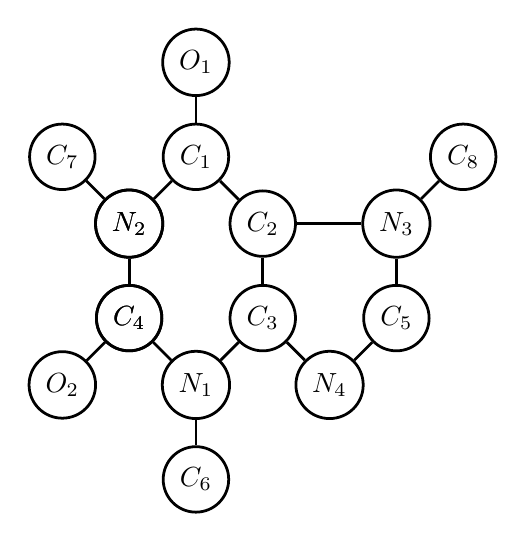
\begin{tikzpicture}[node distance={12mm}, line width=1pt, main/.style = {draw, circle}] 
\node[main] (1) []{$C_1$}; 
\node[main] (2) [below right of=1]{$C_2$}; 
\node[main] (3) [below of=2]{$C_3$}; 
\node[main] (4) [below left of=3]{$N_1$}; 
\node[main] (5) [above left of=4]{$C_4$}; 
\node[main] (6) [above of=5]{$N_2$};
\node[main] (9) [below right of=3]{$N_4$}; 
\node[main] (8) [above right of=9]{$C_5$}; 
\node[main] (7) [above of=8]{$N_3$}; 
\node[main] (10) [above of=1]{$O_1$}; 
\node[main] (11) [above left of=4]{$C_4$}; 
\node[main] (12) [above of=5]{$N_2$}; 

\node[main] (13) [below of=4]{$C_6$};  

\node[main] (17) [below left of=5]{$O_2$};

\node[main] (18) [above left of=6]{$C_7$}; 

\node[main] (22) [above right of=7]{$C_8$}; 



\draw [] (1) -- (2); 
\draw [] (2) -- (3); 
\draw [] (3) -- (4); 
\draw [] (4) -- (5); 
\draw [] (5) -- (6); 
\draw [] (6) -- (1); 
\draw [] (2) -- (7); 
\draw [] (7) -- (8); 
\draw [] (8) -- (9); 
\draw [] (9) -- (3); 
\draw [] (1) -- (10); 

\draw [] (4) -- (13); 

\draw [] (5) -- (17); 

\draw [] (6) -- (18); 

\draw [] (7) -- (22); 
\end{tikzpicture}
% \end{center}
}}
		\quad
		\subfloat[][A Path Decomposition]{\resizebox{0.16\textwidth}{!}{% !TEX root = ../main.tex
% \begin{center}
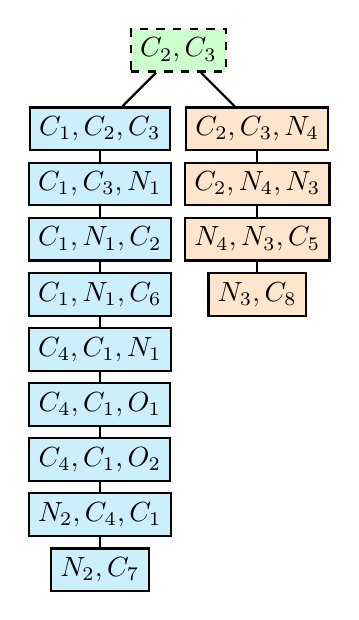
\begin{tikzpicture}[node distance={7mm}, thick, main/.style = {draw, rectangle}] 
\node[main, fill=green!20, dashed] at (0,0) (8) {$C_2,C_3$};
\node[main,fill=cyan!20] at (-1,-1) (7){$C_1,C_2,C_3$};
\node[main,fill=cyan!20] (100) [below of =7] {$C_1,C_3,N_1$};
\node[main,fill=cyan!20] (6) [below of =100]{$C_1,N_1,C_2$};
\node[main,fill=cyan!20] (5) [below of =6]{$C_1,N_1,C_6$};
\node[main,fill=cyan!20] (4) [below of =5]{$C_4,C_1,N_1$};
\node[main,fill=cyan!20] (3) [below of =4]{$C_4,C_1,O_1$};
\node[main,fill=cyan!20] (2) [below of =3]{$C_4,C_1,O_2$};
\node[main,fill=cyan!20] (1) [below of =2]{$N_2,C_4,C_1$};
\node[main,fill=cyan!20] (0) [below of =1] {$N_2,C_7$}; 

%\node[main,white] (00) [right = 1cm of 0] {}; 
%\node[main,white] (000) [left = 1cm of 0] {}; 



\node[main,fill=orange!20] at (1, -1) (9){$C_2,C_3,N_4$};
\node[main,fill=orange!20] (10) [below of =9]{$C_2,N_4,N_3$};
\node[main,fill=orange!20] (11) [below of =10]{$N_4,N_3,C_5$};
\node[main,fill=orange!20] (12) [below of =11]{$N_3, C_8$};


\draw [] (0) -- (1); 
\draw [] (1) -- (2); 
\draw [] (2) -- (3); 
\draw [] (3) -- (4); 
\draw [] (4) -- (5); 
\draw [] (5) -- (6); 
\draw [] (6) -- (100); 
\draw [] (7) -- (100); 
\draw [] (7) -- (8); 
\draw [] (8) -- (9); 
\draw [] (9) -- (10); 
\draw [] (10) -- (11); 
\draw [] (11) -- (12); 


\end{tikzpicture}
% \end{center}}}
		\quad
		\subfloat[][A Tree Decomposition]{\resizebox{0.3\textwidth}{!}{% \begin{center}
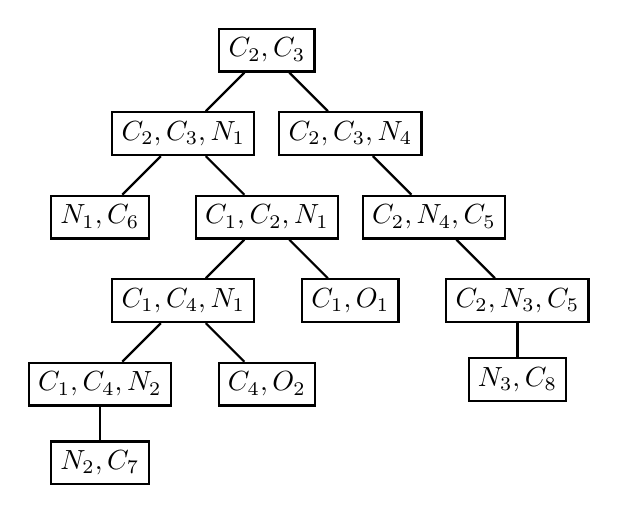
\begin{tikzpicture}[node distance={15mm}, thick, main/.style = {draw, rectangle}] 
\node[main] (0) []{$C_2,C_3$}; 
\node[main] (00) [below left of =0]{$C_2,C_3,N_1$};
\node[main] (000) [below left of =00]{$N_1,C_6$};
\node[main] (001) [below right of =00]{$C_1,C_2,N_1$};
\node[main] (0011) [below right of =001]{$C_1,O_1$};
\node[main] (0010) [below left of =001]{$C_1,C_4,N_1$};
\node[main] (00101) [below right of =0010]{$C_4,O_2$};
\node[main] (00100) [below left of =0010]{$C_1,C_4,N_2$};
\node[main] (001000) [below of =00100,,node distance={10mm}]{$N_2,C_7$};
\node[main] (01) [below right of =0]{$C_2,C_3,N_4$};
\node[main] (011) [below right of =01]{$C_2,N_4,C_5$};
\node[main] (0111) [below right of =011]{$C_2,N_3,C_5$};
\node[main] (01110) [below of =0111,,node distance={10mm}]{$N_3,C_8$};

\draw [] (0) -- (00); 
\draw [] (00) -- (000); 
\draw [] (00) -- (001); 
\draw [] (001) -- (0010); 
\draw [] (001) -- (0011); 
\draw [] (0010) -- (00100); 
\draw [] (00100) -- (001000);  
\draw [] (0010) -- (00101); 

\draw [] (0) -- (01); 
\draw [] (01) -- (011); 
\draw [] (011) -- (0111); 
\draw [] (0111) -- (01110); 

\end{tikzpicture}
% \end{center}}}
		\caption{A Graph Representation of Caffeine and a path and tree decomposition of this graph. Vertices in the root bag of the tree decomposition are highlighted in green (dashed). Notice how the removal of these nodes in the original molecule separates it into two connected components, each corresponding to one of the sides of the path decomposition, and one of the highlighted subtrees in the tree decomposition.}
		\label{fig:tree_dec_caffeine}
	\end{figure}

\end{example}
% \begin{figure}[H]
% 	\centerin{}g
% 	\chemfig{=^[:270](-[:330]=^[:30]-[:90]=^[:150]-[:210])-[:210]=_[:270](%
-[:330]=_[:30]-[:330]=_[:270]-[:210]=_[:150]-[:90])-[:210](-[:270]=_[:330]%
-[:270]=_[:210]-[:150]=_[:90]-[:30])=_[:150](-[:210]=_[:270]-[:210]=_[:150]%
-[:90]=_[:30]-[:330])-[:90](-[:150]=^[:90]-[:150]=^[:210]-[:270]=^[:330]%
-[:30])=_[:30](-[:330])-[:90]=^[:30]-[:90]=^[:150]-[:210]=^[:270](-[:330])}

% 	\caption{1,2,3,4,5,6-hexakis-phenylbenzene}
% 	\label{fig:tw_2 example}
% \end{figure}

\begin{lemma}[Proof in~\ref{app:proof}]\label{intseplemma}
	If $b$ is an introduce node with a single child $c$ and $X_b = X_c \cup \{v\}$, then $N(v)\cap G_b^\downarrow \subseteq X_c$. Here, $N(v)$ is the set of neighbors of $v.$
\end{lemma}



\begin{lemma}[Proof in~\ref{app:proof}]\label{joinseplemma}
	If $b$ is a join node with two children $c_1$ and $c_2,$ then in $G_b^\downarrow$ there is no edge with one endpoint in $V(G_{c_1}^\downarrow) \setminus X_b$ and the other in $V(G_{c_2}^\downarrow) \setminus X_b.$ Informally, $X_b$ is a cut that separates $V(G_{c_1}^\downarrow)$ from $V(G_{c_2}^\downarrow)$ in $G.$ See Figure~\ref{fig:tree_dec_caffeine}.
\end{lemma}

% \begin{proof}
% Let $T^\prime, T^{\prime\prime}, T^{\prime\prime\prime}$ be the subtrees of $T$ rooted at $b, c_1, c_2$ respectively. Let 
% $\mathcal{T}^\prime, \mathcal{T}^{\prime\prime}, \mathcal{T}^{\prime\prime\prime}$ be the corresponding tree decompositions. We will prove the given statement by contradiction. Therefore, let us assume that $u \in V(G_{c_1}^\downarrow) \setminus X_b$, $v \in V(G_{c_2}^\downarrow) \setminus X_b$, and $uv \in E(G_b^\downarrow)$.

% As $\mathcal{T}^{\prime}$ is a tree decomposition of $G^\downarrow_b$, there exists at least one bag $X_t$, such that $t \in \mathcal{T}^{\prime}$ and $u,v \in X_t$. From our initial assumption, we know that $u, v \notin X_b$, this implies that $t \neq b$. Therefore, either $t \in T^{\prime\prime}$ or $t \in T^{\prime\prime\prime}$. Without loss of generality, let us assume that $t \in T^{\prime\prime}$. As $v \in V(G_{c_2}^\downarrow) \setminus X_b$, there exists at least one bag $X_s$ such that, $ s \in T^{\prime\prime\prime}$ and $v \in X_s$. Observe that $v$ appears in both bags $X_s$ and $X_t$. Now by Definition \ref{def:tree_dec}, we know that $T^\prime_{v}$ is a connected subtree and any path connecting $s$ and $t$ goes through $b$. This implies that $X_b \in T^\prime_v$ and $v \in X_b$. This contradicts our initial assumption that $v \notin X_b$, hence completes the proof.
% \end{proof}